\documentclass{beamer}
% \usetheme{Berkeley}
% \usetheme{Madrid}
\usetheme{Warsaw}

\usepackage{amsmath} 
\usepackage{xcolor}
\usepackage{xeCJK}
\setCJKmainfont{WenQuanYi Micro Hei Mono}


\title{机器学习基本原理与实践}
\author{王超}
\institute{}
\date{\today}


\begin{document}

% Frame 0
\frame{\titlepage}
% \frame{\tableofcontents}


% Frame 1
\begin{frame} {机器学习的两大基本问题} 

\begin{block}{分类问题(Classification)}
    {
    程序输出: N维向量(对应N种可能的分类对象的概率, 例如[Dog: 0.75, Cat: 0.20, Duck: 0.05])
    \begin{figure}
    \begin{center}
    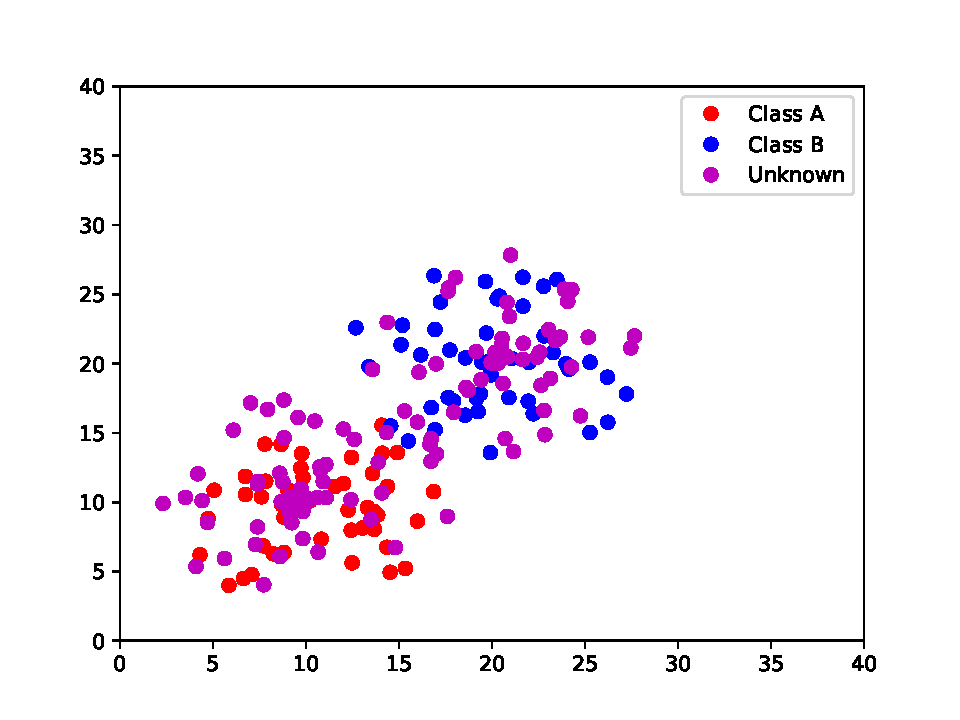
\includegraphics[width=0.4\textwidth]{fig/classification.pdf}
    \end{center}
    \end{figure}
    输入参数: 点的坐标${[x_i, y_i]}$ \\
    输出参数: 分类${[P_A\mbox{(属于A类的概率)}, P_B\mbox{(属于B类的概率)}]}$
    }
\end{block}

\end{frame}



% Frame 2
\begin{frame} {机器学习的两大基本问题} 

\begin{block}{回归问题(Regression), 即求值}
    {
    程序输出: 标量
    \begin{figure}
    \begin{center}
    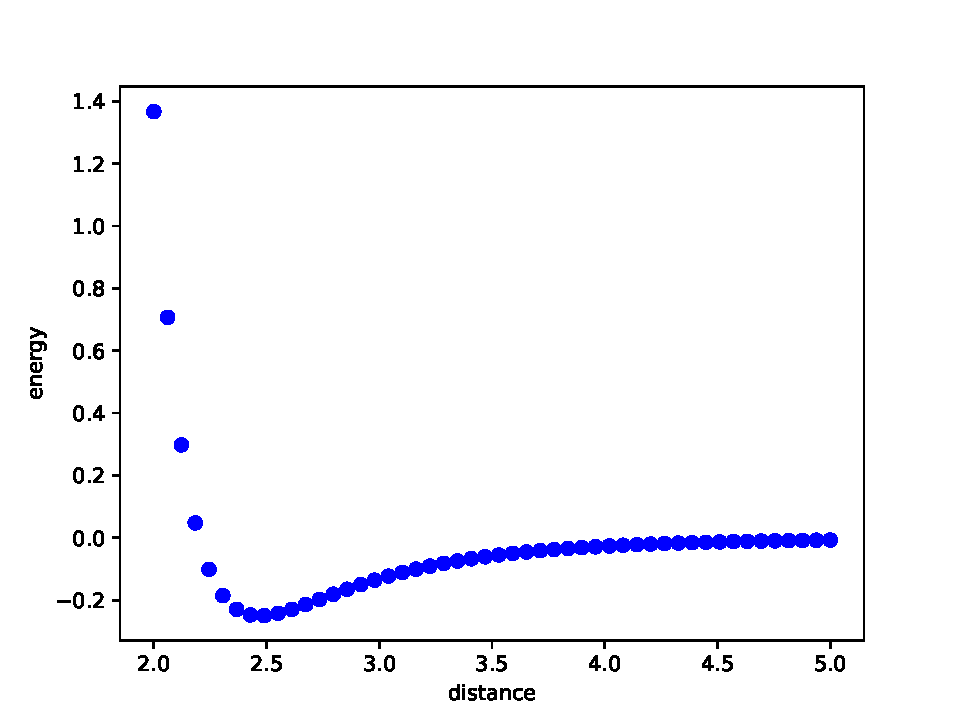
\includegraphics[width=0.4\textwidth]{fig/regression.pdf}
    \end{center}
    \end{figure}
    输入参数: 原子间距离$distance$ \\
    输出参数: 能量$energy$
    }
\end{block}

\end{frame}



% Frame 3
\begin{frame} {机器学习的基本原理: 特征提取+模型拟合} 

\begin{block}{原理: $\mbox{\color{red}原始数据}\xrightarrow{\mbox{特征提取}}\mbox{\color{red}特征}
                    \xrightarrow{\mbox{模型(人工神经网络等)拟合}}\mbox{\color{red}结果}$}
    {
    举例: 卷积神经网络
    \begin{figure}
    \begin{center}
    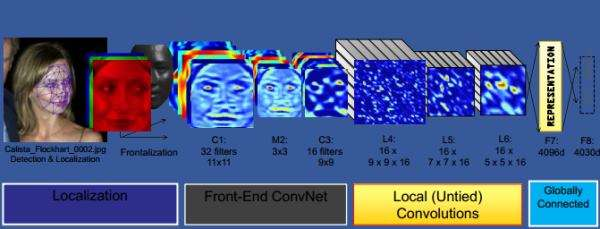
\includegraphics[width=0.6\textwidth]{fig/CNN.png}
    \caption{卷积神经网络人脸识别}
    \end{center}
    \end{figure}
    }
\end{block}

\end{frame}



% Frame 4
\begin{frame} {人工神经网络 Atificial Neutral Network} 

\begin{block}{本质: \mbox{\color{yellow}特征向量内部存在关联}的\mbox{\color{red}非线性}的数学映射}
    \mbox{\underline{线性}的神经网络}
    $${
    \begin{bmatrix}
    r_{00}&r_{01}&r_{02}\\
    r_{10}&r_{11}&r_{12}\\
    r_{20}&r_{21}&r_{22}
    \end{bmatrix} \times
    \begin{bmatrix}
    w_0\\w_1\\w_2
    \end{bmatrix} +
    \begin{bmatrix}
    b
    \end{bmatrix} =
    \begin{bmatrix}
    r_{00} \cdot w_0+r_{01}w_1+r_{02}w_2+b \\
    r_{10} \cdot w_0+r_{11}w_1+r_{12}w_2+b \\
    r_{20} \cdot w_0+r_{21}w_1+r_{22}w_2+b \\
    \end{bmatrix}
    \
    }$$
    $\begin{bmatrix}r_{i0}&r_{i1}&r_{i2}\end{bmatrix}$是第$i$个样本的特征向量 \\
    $\begin{bmatrix}w_0\\w_1\\w_2\end{bmatrix}$是权重因子,表征各个特征对输入结果的贡献大小 \\
    $\begin{bmatrix}b\end{bmatrix}$是偏置因子 
    \begin{center}
    \boxed{\mbox{本质是线性变换$y=w \cdot x+b$}}
    \end{center}
\end{block}

\end{frame}



% frame 5
\begin{frame} {人工神经网络 Atificial Neutral Network} 

\begin{block}{本质: \mbox{\color{yellow}特征向量内部存在关联}的\mbox{\color{red}非线性}的数学映射}
    \mbox{\underline{非线性}的神经网络}
    $${
    \begin{bmatrix}
    r_{00}&r_{01}&r_{02}\\
    r_{10}&r_{11}&r_{12}\\
    r_{20}&r_{21}&r_{22}
    \end{bmatrix} \times
    \begin{bmatrix}
    w_0\\w_1\\w_2
    \end{bmatrix} +
    \begin{bmatrix}
    b
    \end{bmatrix} =
    \begin{bmatrix}
    r_{00} \cdot w_0+r_{01}w_1+r_{02}w_2+b \\
    r_{10} \cdot w_0+r_{11}w_1+r_{12}w_2+b \\
    r_{20} \cdot w_0+r_{21}w_1+r_{22}w_2+b \\
    \end{bmatrix}
    }$$
    $${
    \xrightarrow[sin() \quad tanh() \quad relu() \quad...]{\mbox{激活函数Activation Function}}
    \begin{bmatrix}
    f_{act}(r_{00} \cdot w_0+r_{01}w_1+r_{02}w_2+b) \\
    f_{act}(r_{10} \cdot w_0+r_{11}w_1+r_{12}w_2+b) \\
    f_{act}(r_{20} \cdot w_0+r_{21}w_1+r_{22}w_2+b) \\
    \end{bmatrix}    
    }$$
    
    \begin{center}
    \boxed{\mbox{通过激活函数引入非线性,增强模型的刻画能力}}
    \end{center}
\end{block}

\end{frame}



% frame 6
\begin{frame} {人工神经网络 Atificial Neutral Network} 

\begin{block}{人工神经网络的训练}
    人工神经网络模型的训练的本质是通过优化
    $\begin{bmatrix}w_0\\w_1\\w_2\end{bmatrix}$和$\begin{bmatrix}b\end{bmatrix}$
    使神经网络的输出值与真实值趋于一致,从而实现对未知特征的预测
\end{block}

\end{frame}


\end{document}